\documentclass[10pt, oneside]{book}
\usepackage{xeCJK}
\usepackage{amsmath, amsthm, amssymb, bm, graphicx, hyperref, mathrsfs}
\usepackage{geometry}
% \geometry{b5paper,scale=0.85}
\geometry{b5paper,left=1.2cm,right=1.2cm,top=2cm,bottom=1cm}
\usepackage{graphicx} %插入图片的宏包
\usepackage{float} %设置图片浮动位置的宏包
\usepackage{subfigure} %插入多图时用子图显示的宏包
\usepackage{amstext} %公式中包含文字的宏包
\usepackage{booktabs} %插入表格的宏包
\usepackage{multirow} 
\usepackage{indentfirst} %设置缩进的宏包
\setlength{\parindent}{2em}
\usepackage{enumerate} %用于编号的宏包
\usepackage{hyperref} %用于引用的宏包
% \hypersetup{colorlinks, linkcolor=blue} %设置引用的字体颜色



% 封面部分
\title{\Huge{\textbf{ROS Notebook}}}
\author{Wu Yutian}
\date{2021.11.13}
\linespread{1.4}
\newtheorem{theorem}{定理}[section]
\newtheorem{definition}[theorem]{定义}
\newtheorem{lemma}[theorem]{引理}
\newtheorem{corollary}[theorem]{推论}
\newtheorem{example}[theorem]{例}
\newtheorem{proposition}[theorem]{命题}
\begin{document}

% 输出封面
\maketitle

% 前言部分
\pagenumbering{roman}
\setcounter{page}{1}

\begin{center}
    \Huge\textbf{前言}
\end{center}~\

主要参考了胡春旭的《ROS机器人开发实践》一书。

~\\
\begin{flushright}     
    \begin{tabular}{c}
        Wu Yutian\\
        2021.11.13
    \end{tabular}
\end{flushright}

\newpage
\pagenumbering{Roman}
\setcounter{page}{1}
\tableofcontents
\newpage
\setcounter{page}{1}
\pagenumbering{arabic}

% -------------------------chapter 1-------------------------
\chapter{ROS的基本架构——ROS1}

\section{整体架构}

\begin{figure}[H]
    \centering
    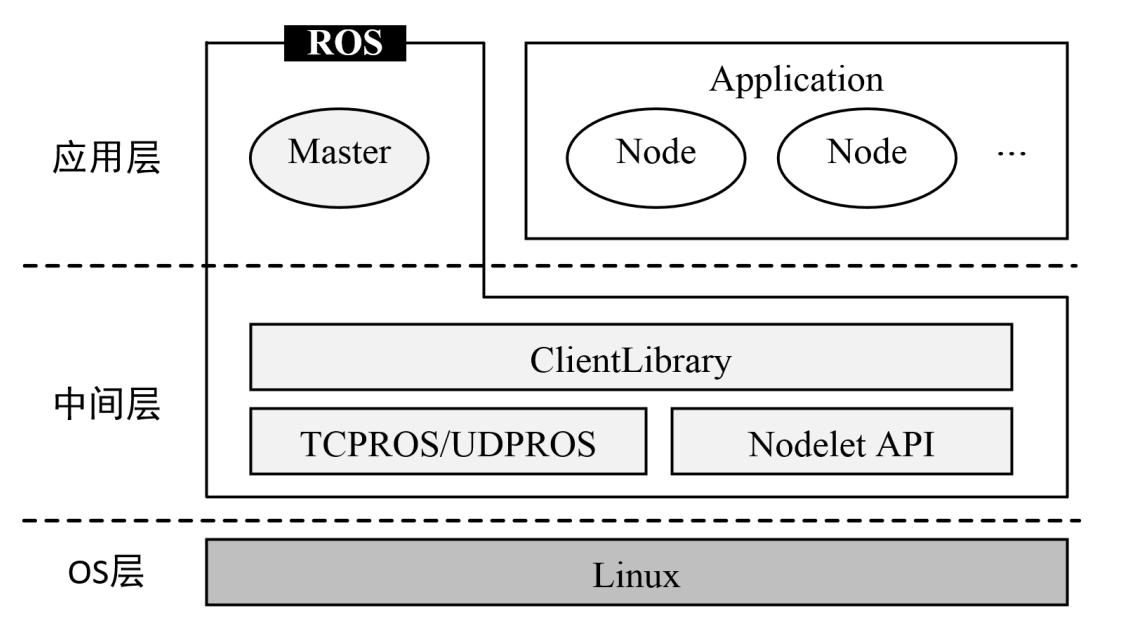
\includegraphics[width=0.6\linewidth]{image/ROS1架构.jpg}
\end{figure}

OS层:是ROS依托的底层操作系统,一般是Ubuntu。

中间层:最重要的就是基于TCP/UDP网络,进行封装形成的TCPROS/UDPROS通信系统,这其中包括了Topic的发布、订阅的通信方式,Service的客户端、服务器的通信方式等。另外ROS还提供了一种进程内通信的方式——Nodelet,可以为多进程通信提供一种更优化的数据传输方式,适合对实时性要求较高的应用。

在通信机制的基础上,ROS还在中间层提供了大量的机器人开发相关的实用功能,如:数据类型定义、坐标变换、运动控制等。

应用层:ROS需要运行一个管理者——Matser,负责整个系统的正常运行。其他的一些相关的ROS功能包都是以节点(Node)的方式运行,一般来说,简单的开发工作只需要关注节点的标准输入输出接口,而不需要关注模块的内部实现。

\section{计算图的视角}

\begin{figure}[H]
    \centering
    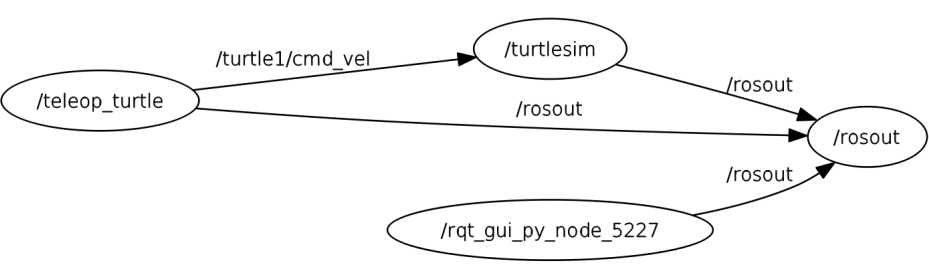
\includegraphics[width=0.7\linewidth]{image/计算图.png}
\end{figure}

从计算图的视角来看ROS的功能模块,它们都是以节点为单位独立运行的,甚至可以分布于不同的主机中。

\subsection{节点 Node}

节点就是一些执行运算任务的进程,它们之间可以相互通信。

\subsection{话题 Topic}

消息以一种发布/订阅(publish/subscribe)的方式传递,发布者和订阅者并不了解彼此的存在,系统中可能有多个节点发布或者订阅同一个话题的消息。

\subsection{服务 Service}

对于双向的同步传输模式,采用基于客户端/服务器(Client/Server)的模型,包含请求和应答,类似于Web服务器,ROS中只允许有一个节点提供指定命名的服务。

\subsection{节点管理器 Master}

节点管理器帮助ROS节点之间相互查找、建立连接,同时还为系统提供参数服务器,管理全局参数。

\section{文件系统}

\subsection{功能包}

功能包相关的常用ROS命令:

\begin{table}[H]
    \centering
    \begin{tabular}{c|c}
    \hline
    命令                  & 作用            \\ \hline
    catkin\_create\_pkg & 创建功能包         \\
    rospack             & 获取功能包的信息      \\
    catkin\_make        & 编译功能包的信息      \\
    rosdep              & 自动安装功能包依赖的其他包 \\
    roscd               & 功能包目录跳转       \\
    roscp               & 拷贝功能包中的文件     \\
    rosed               & 编辑功能包中的文件     \\
    rosrun              & 运行功能包中的可执行文件  \\
    roslaunch           & 运行启动文件        \\ \hline
    \end{tabular}
\end{table}

\section{通信机制}

\subsection{话题通信机制——Topic}

\begin{figure}[H]
    \centering
    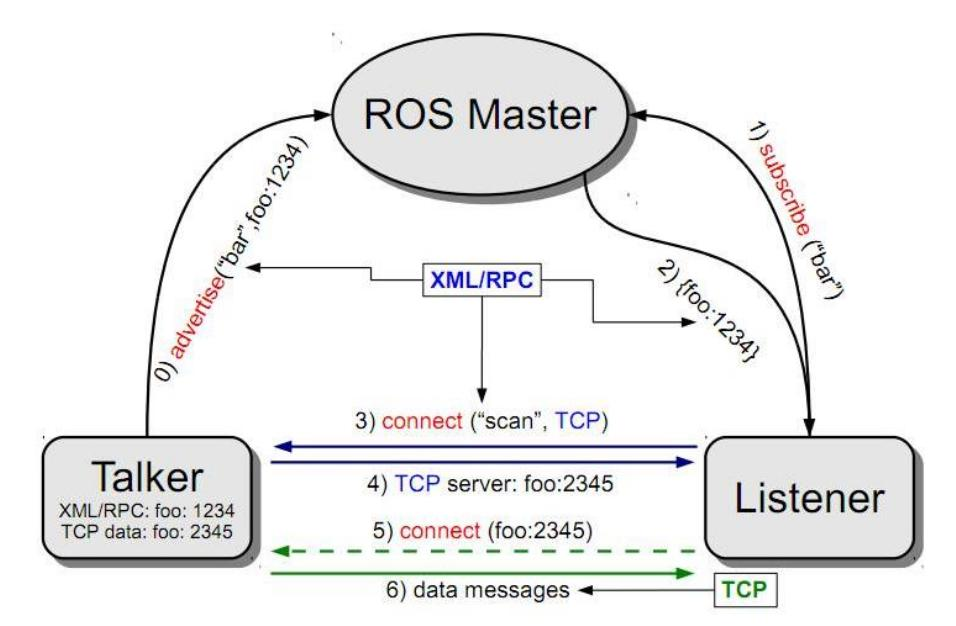
\includegraphics[width=0.7\linewidth]{image/话题通信机制.jpg}
\end{figure}

假设Talker首先启动,建立通信的详细过程:

\begin{itemize}
    \item 1、发布者(Talker)启动,通过RPC向 ROS Master 注册发布者的信息,包括:发布者节点信息,话题名,话题缓存大小等;Master 会将这些信息加入注册列表中;
    \item 2、订阅者(Listener)启动,通过 RPC 向 ROC Master 注册订阅者信息,包括:订阅者节点信息,话题名等;Master 会将这些信息加入注册列表;
    \item 3、Master 进行节点匹配:Master 会根据订阅者提供的信息,在注册列表中查找匹配的发布者;如果没有发布者(Talker),则等待发布者(Talker)的加入;如果找到匹配的发布者(Talker),则会主动把发布者(Talker)(有可能是很多个 Talker)的地址通过 RPC 传送给订阅者(Listener)节点;
    \item 4、Listener 接收到 Master 的发出的 Talker 的地址信息,尝试通过 RPC 向 Talker 发出连接请求(信息包括:话题名,消息类型以及通讯协议(TCP/UDP));
    \item 5、Talker 收到 Listener 发出的连接请求后,通过 RPC 向 Listener 确认连接请求(包含的信息为自身 TCP 地址信息);
    \item 6、Listener 接收到 Talker 的确认消息后,使用 TCP 尝试与 Talker 建立网络连接;
    \item 7、成功连接之后,Talker 开始向 Listener 发布话题消息数据;
\end{itemize}

需要注意的是:有可能多个 Talker 连接一个 Listener,也有可能是一个 Talker 连接上多个 Listener(多对多)。

\subsection{服务通信机制——Service}

\begin{figure}[H]
    \centering
    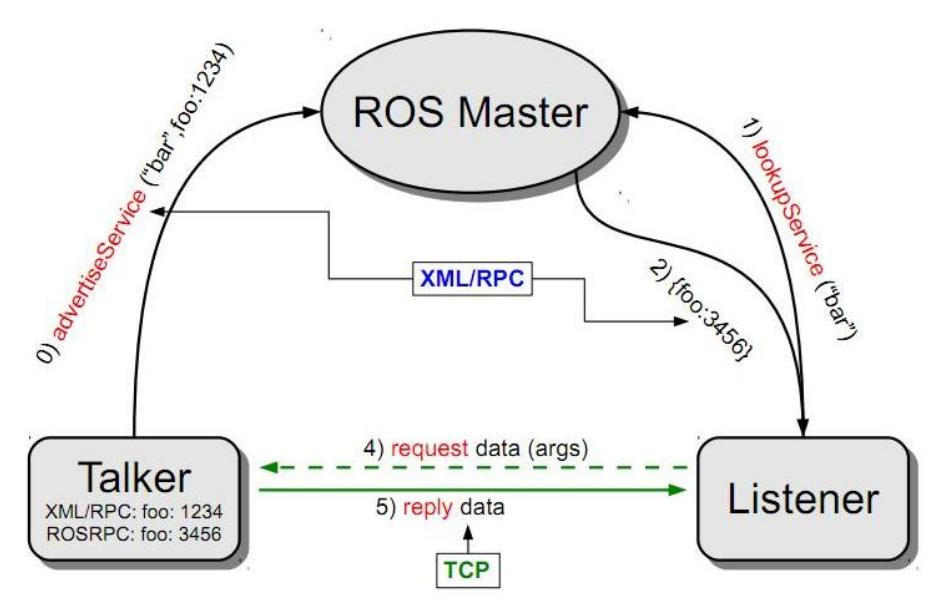
\includegraphics[width=0.7\linewidth]{image/服务通信机制.jpg}
\end{figure}

与话题的通信相比,其减少了Listener与Talker之间的RPC通信,建立通信的详细过程:

\begin{itemize}
    \item 1、发布者(Talker)启动,通过RPC向 ROS Master 注册发布者的信息,包括:发布者节点信息,话题名,话题缓存大小等;Master 会将这些信息加入注册列表中;
    \item 2、订阅者(Listener)启动,通过 RPC 向 ROC Master 注册订阅者信息,包括:订阅者节点信息,话题名等;Master 会将这些信息加入注册列表;
    \item 3、Master 进行节点匹配:Master 会根据订阅者提供的信息,在注册列表中查找匹配的发布者;如果没有发布者(Talker),则等待发布者(Talker)的加入;如果找到匹配的发布者(Talker),则会主动把发布者(Talker)(有可能是很多个 Talker)的地址通过 RPC 传送给订阅者(Listener)节点;
    \item 4、Listener 接收到 Talker 的确认消息后,使用 TCP 尝试与 Talker 建立网络连接;
    \item 5、成功连接之后,Talker 开始向 Listener 发布话题消息数据;
\end{itemize}

需要注意的是:有可能是一个 Talker 连接上多个 Listener(一对多)。

\subsection{参数管理机制——Parameter}

\begin{figure}[H]
    \centering
    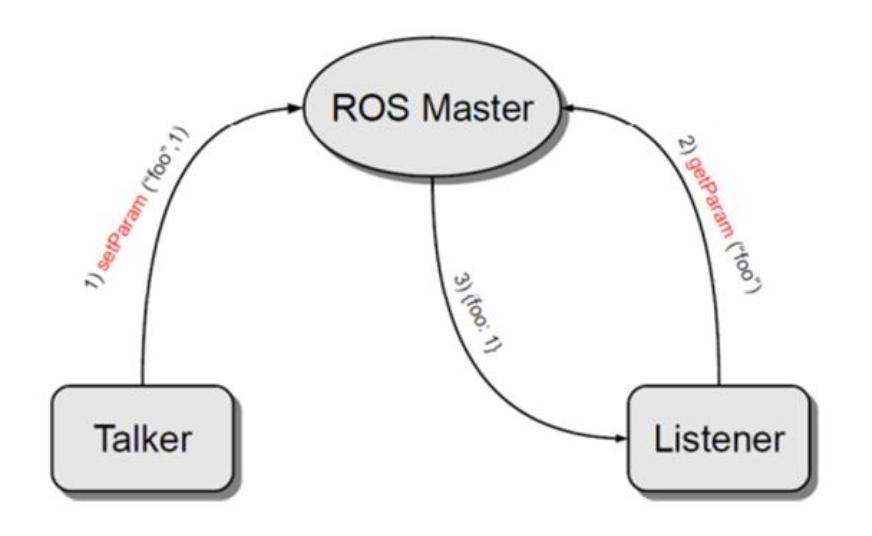
\includegraphics[width=0.7\linewidth]{image/参数管理机制.jpg}
\end{figure}

参数共享机制类似于程序中的全局变量,Talker 去更新全局变量(共享的参数),Listener 去获取更新后的全局变量(共享的参数);这个通信过程不涉及 TCP/UDP 的通信;     

\begin{itemize}
    \item 1、Talker 更新全局变量;Talker 通过 RPC 更新 ROS Master 中的共享参数(包含参数名和参数值);
    \item 2、Listener 通过 RPC 向 ROS Master 发送参数查询请求(包含要查询的参数名);
    \item 3、ROS Master 通过 RPC 回复 Listener 的请求(包括参数值);
\end{itemize}

需要注意的是:如果 Listener 向实时知道共享参数的变化,需要自己不停的去询问 ROS Master;


% -------------------------chapter 2-------------------------
\chapter{ROS基础}

\section{turtlesim功能包}

接触的第一个ROS功能包:turtlesim,其核心是tuetlesim\_node节点。

其中包含的话题和服务如下:

\begin{table}[H]
    \centering
    \begin{tabular}{ccll}
    \hline
                                             & 名称                                               & \multicolumn{1}{c}{类型}                                                                      & \multicolumn{1}{c}{描述}                                                \\ \hline
    \multicolumn{1}{c|}{话题订阅}                & \multicolumn{1}{c|}{turtleX/cmd\_vel}            & \multicolumn{1}{l|}{\begin{tabular}[c]{@{}l@{}}geometry\_msgs/\\ Twist\end{tabular}}        & \begin{tabular}[c]{@{}l@{}}控制乌龟角速度与线速度的\\ 输入指令\end{tabular}           \\ \hline
    \multicolumn{1}{c|}{话题发布}                & \multicolumn{1}{c|}{turtleX/pose}                & \multicolumn{1}{l|}{turtlesim/Pose}                                                         & \begin{tabular}[c]{@{}l@{}}乌龟的姿态信息:包括x与y\\ 坐标、角度、线速度和角速度\end{tabular} \\ \hline
    \multicolumn{1}{c|}{\multirow{7}{*}{服务}} & \multicolumn{1}{c|}{clear}                       & \multicolumn{1}{l|}{std\_srvs/Empty}                                                        & 清楚仿真器中的背景颜色                                                           \\ \cline{2-4} 
    \multicolumn{1}{c|}{}                    & \multicolumn{1}{c|}{reset}                       & \multicolumn{1}{l|}{std\_srvs/Empty}                                                        & 复位仿真器到初始状态                                                            \\ \cline{2-4} 
    \multicolumn{1}{c|}{}                    & \multicolumn{1}{c|}{kill}                        & \multicolumn{1}{l|}{turtlesim/Kill}                                                         & 删除一只乌龟                                                                \\ \cline{2-4} 
    \multicolumn{1}{c|}{}                    & \multicolumn{1}{c|}{spawn}                       & \multicolumn{1}{l|}{turtlesim/Spawn}                                                        & 新生一只乌龟                                                                \\ \cline{2-4} 
    \multicolumn{1}{c|}{}                    & \multicolumn{1}{c|}{turtleX/set\_pen}            & \multicolumn{1}{l|}{turtlesim/Setpen}                                                       & 设置画笔的颜色和线宽                                                            \\ \cline{2-4} 
    \multicolumn{1}{c|}{}                    & \multicolumn{1}{c|}{turtleX/teleport\_absolute}  & \multicolumn{1}{l|}{\begin{tabular}[c]{@{}l@{}}turtlesim/\\ TeleportAbsolute\end{tabular}}  & 移动乌龟到指定的姿态                                                            \\ \cline{2-4} 
    \multicolumn{1}{c|}{}                    & \multicolumn{1}{c|}{turtleX/teleport\_realative} & \multicolumn{1}{l|}{\begin{tabular}[c]{@{}l@{}}turtlesim/\\ TeleportRealative\end{tabular}} & 移动乌龟到指定的角度和距离                                                         \\ \hline
    \end{tabular}
\end{table}

\section{创建工作空间和功能包}

\subsection{创建工作空间}


工作空间初始化:
\begin{verbatim}
    mkdir ~/catkin_ws/src
    cd ~/catkin_ws/src
    catkin_init_workspace
\end{verbatim}

初始化后,可以编译整个工作空间:
\begin{verbatim}
    cd ~/catkin_ws/
    catkin_make
\end{verbatim}

编译后,在工作空间的根目录下会产生build和devel两个文件夹,在devel文件夹中有setup.bash形式的环境变量设置脚本,则可以使用source命令运行这些脚本配置环境变量,如:
\begin{verbatim}
    source devel/setup.bash
\end{verbatim}

但是source命令设置的环境变量只在当前终端中有效,所以为了方便,可以讲终端的配置文件(~/.bashrc)中加入上面的环境变量的配置语句(要注意写全绝对路径)。

\subsection{创建功能包}

创建功能包的命令如下:

\begin{verbatim}
    cd ~/catkin_ws/src
    catkin_create_pkg <package_name> [depend1] [depend2] [depend3]
\end{verbatim}

创建完成后,工作空间的src目录中会生成一个<package\_name>的功能包,并且已经包含了package.xml和CMakelist.txt文件。其中package.xml文件提供描述功能包属性的信息,CMakelist.txt文件记录功能包的编译规则。

进而可以回到工作空间的根目录下进行编译,并设置环境变量。

\section{工作空间的覆盖}

所有工作空间的路径会依次在ROS\_PACKAGE\_PATH环境变量中记录,当设置多个工作空间的环境变量后,新设置的路径在ROS\_PACKAGE\_PATH中会自动放在最前端。在运行时,ROS会优先查找最前端的工作空间中是否存在指定的功能包,如果不存在,就顺序向后查找其他工作空间,知道最后一个工作空间为止。

\section{Topic中的Publisher和Subscriber}

\subsection{Publisher的创建}

\begin{verbatim}
    #include <sstream>
    #include "ros/ros.h"
    #include "std_msgs/String.h"
    int main(int argc, char **argv){
        // ROS节点初始化
        ros::init(argc, argv, "talker");
        // 创建节点句柄
        ros::NodeHandle n;
        // 创建一个Publisher,发布名为chatter的topic,消息类型为std_msgs::String
        ros::Publisher chatter_pub = n.advertise<std_msgs::String>("chatter", 1000);
        // 设置循环的频率
        ros::Rate loop_rate(10);
        int count = 0;
        // 一旦发生异常,ros::ok()就会返回false,跳出循环
        while (ros::ok()){
            // 初始化std_msgs::String类型的消息
            std_msgs::String msg;
            std::stringstream ss;
            ss << "hello world " << count;
            msg.data = ss.str();
            // 发布消息
            ROS_INFO("%s", msg.data.c_str());
            chatter_pub.publish(msg);
            // 循环等待回调函数
            // ros::spinOnce()函数用来处理节点订阅话题的所有回调函数
            // 虽然目前的发布节点并没有任何订阅信息,ros::spinOnce()不是必须的
            // 但是为了保证功能无误,建议所有节点都默认加入该函数
            ros::spinOnce();
            // 按照循环频率延时
            loop_rate.sleep();
            ++count;
        }
        return 0;
    }
\end{verbatim}

\subsection{Subscriber的创建}

\begin{verbatim}
    #include "ros/ros.h"
    #include "std_msgs/String.h"
    // 接收到订阅的消息后,会进入消息回调函数
    // 当有消息到达时,会自动以消息指针作为参数
    void chatterCallback(const std_msgs::String::ConstPtr& msg){
        // 将接收到的消息打印出来
        ROS_INFO("I heard: [%s]", msg->data.c_str());
    }
    int main(int argc, char **argv){
        // 初始化ROS节点
        ros::init(argc, argv, "listener");
        // 创建节点句柄
        ros::NodeHandle n;
        // 创建一个Subscriber,订阅名为chatter的topic,注册回调函数chatterCallback
        ros::Subscriber sub = n.subscribe("chatter", 1000, chatterCallback);
        // 循环等待回调函数
        ros::spin();
        return 0;
    }
\end{verbatim}

\subsection{自定义话题消息}

\subsubsection{编写msg文件}

使用msg文件定义自己的消息类型,一般放置在功能包根目录下的msg文件夹中。msg文件中既可以定义消息类型的变量,也可以定义常量:

\begin{verbatim}
    string name
    uint8  sex
    uint8  age
    
    uint8 unknown = 0
    uint8 male    = 1
    uint8 female  = 2
\end{verbatim}

对于稍复杂一些的ROS自定义消息,还会包含一个标准格式的头信息std\_msgs/Header:
\begin{verbatim}
    unint32 seq
    time stamp
    string frame_id  
\end{verbatim}

其中:seq是消息的顺序标识,不需要手动设置,Publisher在发布消息时会自动累加;stamp是消息中与数据相关联的时间戳,可以用于时间同步;frame\_id是消息中与数据相关联的参考坐标系id。

\subsubsection{编译msg文件}

(1)在package.xml中添加功能包依赖

\begin{verbatim}
    <build_depend>message_generation</build_depend>
    <run_depend>message_runtime</run_depend>
\end{verbatim}

(2)在CMakeLists.txt文件中添加编译选项

在find\_package中添加消息生成依赖的功能包message\_generation:
\begin{verbatim}
    find_package(catkin REQUIRED COMPONENTS
        geometry_msgs
        roscpp
        rospy
        std_msgs
        message_generation
    )
\end{verbatim}

设置catkin依赖:
\begin{verbatim}
    catkin_package(
        # INCLUDE_DIRS include
        # LIBRARIES learning_communication
        CATKIN_DEPENDS geometry_msgs roscpp rospy std_msgs message_runtime
        # DEPENDS system_lib
    )
\end{verbatim}

设置需要编译的msg文件:
\begin{verbatim}
    add_message_files(FILES Person.msg) 
    generate_messages(DEPENDENCIES std_msgs)
\end{verbatim}

然后对功能包进行编译,自定义的消息类型就生效了。

\subsection{CMakeLists的编写}

几个常用的编译选项:

(1)include\_directories

用于设置头文件的相对路径。功能包的一些头文件会放在功能包根目录下的include文件夹中,所以需要添加该文件夹。

(2)add\_executable

用于设置需要编译的代码和生成的可执行文件。第一个参数为期望生成的可执行文件的名称,后面的参数为参与的源码文件(cpp),如果需要多个代码文件,可以在后面依次列出,中间用空格分隔。

(3)target\_link\_libraries

用于设置链接库。第一个参数为期望生成的可执行文件的名称,后面依次列出需要链接的库,如果没有使用其他库,添加默认链接库(\$\{catkin\_LIBRARIES\})即可。

(4)add\_dependencies

用于设置依赖。在很多应用中,我们需要定义语言无关的消息类型,消息类型会在编译过程中产生相应语言的代码,如果编译的可执行文件依赖这些动态生成的代码,则需要使用add\_dependencies添加\$\{PROJECT\_NAME\}\_generate\_messages\_cpp配置,即该功能包动态产生的消息代码。

对于我们的这个例子,CMakeLists.txt文件如下:

\begin{verbatim}
    include_directories(include ${catkin_INCLUDE_DIRS})

    add_executable(talker src/talker.cpp)
    target_link_libraries(talker ${catkin_LIBRARIES})
    add_dependencies(talker ${PROJECT_NAME}_generate_messages_cpp)
      
    add_executable(listener src/listener.cpp)
    target_link_libraries(listener ${catkin_LIBRARIES})
    add_dependencies(talker ${PROJECT_NAME}_generate_messages_cpp)
\end{verbatim}


\section{Service中的Client和Server}

\subsection{创建Client}

\begin{verbatim}
    #include <cstdlib>
    #include "ros/ros.h"
    #include "learning_communication/AddTwoInts.h"
    
    int main(int argc, char **argv){
        ros::init(argc, argv, "add_two_ints_client");
        // 从终端命令行获取两个加数,argv[0]是路径,argv[1]和[2]是两个输入参数
        if (argc != 3){
            ROS_INFO("usage: add_two_ints_client X Y");
            return 1;
        }
        ros::NodeHandle n;    
        // 创建一个client,请求add_two_int service
        // service消息类型是learning_communication::AddTwoInts
        ros::ServiceClient client = n.serviceClient\
            <learning_communication::AddTwoInts>("add_two_ints");
        // 创建learning_communication::AddTwoInts类型的service消息
        // 该变量包含两个成员:request和response
        learning_communication::AddTwoInts srv;
        // atoll()函数将字符串转化为整数
        srv.request.a = atoll(argv[1]);
        srv.request.b = atoll(argv[2]);
        // 发布service请求,等待加法运算的应答结果
        // 调用过程会发生阻塞,调用成功后返回true
        if (client.call(srv)){
            ROS_INFO("Sum: %ld", (long int)srv.response.sum);
        }
        else{
            ROS_ERROR("Failed to call service add_two_ints");
            return 1;
        }
        return 0;
    }
\end{verbatim}

\subsection{创建server}

\begin{verbatim}
    #include "ros/ros.h"
    #include "learning_communication/AddTwoInts.h"
    // service回调函数,输入参数req,输出参数res
    bool add(learning_communication::AddTwoInts::Request  &req,
             learning_communication::AddTwoInts::Response &res){
        // 将输入参数中的请求数据相加,结果放到应答变量中
        res.sum = req.a + req.b;
        ROS_INFO("request: x=%ld, y=%ld", (long int)req.a, (long int)req.b);
        ROS_INFO("sending back response: [%ld]", (long int)res.sum);
        return true;
    }
    int main(int argc, char **argv){
        ros::init(argc, argv, "add_two_ints_server");
        ros::NodeHandle n;
        // 创建一个名为add_two_ints的server,注册回调函数add()
        ros::ServiceServer service = n.advertiseService("add_two_ints", add);
        // 循环等待回调函数
        ROS_INFO("Ready to add two ints.");
        ros::spin();
        return 0;
    }    
\end{verbatim}

\subsection{自定义服务数据}

\subsubsection{编写srv文件}

使用 srv 文件定义自己的消息类型,一般放置在功能包根目录下的 srv 文件夹中。该文件包含request和response两个数据域,两个数据域之间用"---"(三个减号)分隔,如:

\begin{verbatim}
    int64 a
    int64 b
    ---
    int64 sum
\end{verbatim}

\subsubsection{编译srv文件}

(1)在 package.xml 中添加功能包依赖(与自定义话题消息相同)

\begin{verbatim}
    <build_depend>message_generation</build_depend>
    <run_depend>message_runtime</run_depend>
\end{verbatim}

(2)在CMakeLists.txt文件中添加编译选项

与自定义话题消息相同也是添加message\_generation包,

\begin{verbatim}
    find_package(catkin REQUIRED COMPONENTS
        geometry_msgs
        roscpp
        rospy
        std_msgs
        message_generation
    )
    add_service_files(FILES AddTwoInts.srv)
\end{verbatim}

\subsection{CMakeLists的编写}

与Topic类似:

\begin{verbatim}
    include_directories(include ${catkin_INCLUDE_DIRS})
            
    add_executable(server src/server.cpp)
    target_link_libraries(server ${catkin_LIBRARIES})
    add_dependencies(server ${PROJECT_NAME}_gencpp)

    add_executable(client src/client.cpp)
    target_link_libraries(client ${catkin_LIBRARIES})
    add_dependencies(client ${PROJECT_NAME}_gencpp)
\end{verbatim}

\section{ROS中的命名空间}

\subsection{有效的命名}

\begin{itemize}
    \item 1、首字符必须是([a-z|A-Z])、波浪线(\textasciitilde)或者左斜杠(/)
    \item 2、后续字母可以是字母或数字([0-9|a-z|A-Z])、下划线(\_)或者左斜杠
\end{itemize}

\subsection{命名解析}

\subsubsection{全局名称:/global/name}

全局名称的首字符是左斜杠,它之所以称为全局,是因为它的解析度最高,可以在全局范围内直接访问。

但是在系统中,全局名称越少越好,因为过多的全局名称会影响功能包的可移植性。

\subsubsection{相对名称:relative/name}

相对名称由ROS提供默认的命名空间,不需要带有开头的左斜杠,ROS会对一个相对名称进行解析,进而得到一个全局名称来使用,就类似与我们平时使用的相对路径。相对名称的使用会提高可移植性。

例如:在默认命名空间/relative内使用相对名称name,则系统会将其解析为全局名称:/relative/name。

ROS提供的三种指定默认命名空间的方式:

\begin{itemize}
    \item[-] 1、通过命令参数设置

    调用ros::init()的程序会接受一个名为\_\_ns的命令行参数,用来设置默认命名空间:

\begin{verbatim}
__ns:=deflaut-namespace
\end{verbatim}

    \item[-] 2、在launch文件中设置
    
    在launch文件中可以通过参数ns来设置默认命名空间:

\begin{verbatim}
<node pkg="turtlesim" type="turtlesim_node" name="turtlesim\_node" ns="sim1"/>
\end{verbatim}

    \item[-] 3、使用环境变量设置
    
    在执行ROS程序的终端中设置默认命名空间的环境变量:

\begin{verbatim}
export ROS_NAMESPACE = default-namespace
\end{verbatim}


\end{itemize}

\subsubsection{私有名称:~private/name}

私有名称是一个节点内部私有的资源名称,只会在节点内部使用。私有名称以波浪线“\textasciitilde”开始。类似相对名称,也需要ROS为其解析,成为一个有意义的全局名称,不同的是,私有名称并不使用当前的默认命名空间,而是使用节点的全局名称作为命名空间。

例如有一个节点的全局名称是/sim1/pubvel,其中的一个私有名称为\textasciitilde/max\_vel,则其会被解析成全局名称:/sim1/pubvel/max\_vel。

\subsubsection{ROS命名解析总结}

\begin{table}[H]
    \begin{tabular}{c|c|c|c}
    \hline
    节点        & 全局名称                            & 相对名称(默认)                         & 私有名称                                         \\ \hline
    /node1    & /bar -\textgreater /bar         & Bar -\textgreater /bar           & $\sim$bar -\textgreater /node1/bar           \\ \hline
    /wg/node2 & /bar -\textgreater /bar         & Bar -\textgreater /wg/bar        & $\sim$bar -\textgreater wg/node2/bar         \\ \hline
    /wg/node3 & /foo/bar -\textgreater /foo/bar & foo/bar -\textgreater wg/foo/bar & $\sim$foo/bar -\textgreater wg/node3/foo/bar \\ \hline
    \end{tabular}
\end{table}

\subsection{命名重映射}

所有的ROS节点内的资源名称都可以在节点启动的时候进行重映射,这一特性支持我们同事打开多个相同的节点,而不会发生命名冲突。

命名重映射语法:

\begin{verbatim}
    old\_name:=new\_name
\end{verbatim}

例如,要将chatter重映射为/wg/chatter,在节点启动时候可以输入如下命令:

\begin{verbatim}
    $ rosrun rospy_tutorials talker chatter:=/wg/chatter 
\end{verbatim}

需要注意:ROS的命名解析是在命名重映射之前发生的。所以当我们使用“foo:=bar”时,会将节点内所有foo命名映射为bar,而如果我们重映射“/foo:=bar”时,ROS只会讲全局解析为/foo的名称重映射为bar。

命名重映射和命名解析之间的关系:

\begin{table}[H]
    \centering
    \begin{tabular}{c|c|c|c}
    \hline
    节点命名空间 & 重映射参数            & 匹配名称         & 解析名称       \\ \hline
    /      & foo:=bar         & foo,/foo     & /bar       \\ \hline
    /baz   & foo:=bar         & foo,/baz/foo & /baz/bar   \\ \hline
    /      & /foo:=bar        & foo,/foo     & /bar       \\ \hline
    /baz   & /foo:=bar        & /foo         & /baz/bar   \\ \hline
    /baz   & /foo:=/a/b/c/bar & /foo         & /a/b/c/bar \\ \hline
    \end{tabular}
\end{table}

\section{多机通信}

\subsubsection{设置IP地址}

\begin{itemize}
    \item 1、确保所有计算机处于同一网络中,使用ifconfig命令查看本机的局域网ip地址。
    \item 2、分别在每台计算机的/etc/hosts文件中添加其他计算机的ip地址和对应的计算机名称。
    \item 3、测试是否能够ping通其他计算机。
\end{itemize}

\subsubsection{设置ROS\_MASTER\_URI}

因为系统中只能存在一个Master,所以从机需要知道Master的位置,可以在从机中使用如下命令,将Master的地址写入环境变量中:

\begin{verbatim}
    $ echo "export ROS_MASTER_URI = http://<主机名>::11311" >> ~/.bashrc
\end{verbatim}


% -------------------------chapter 3-------------------------
\chapter{ROS中的常用组件}

\section{launch文件}

launch文件是ROS中同时启动多个节点的途径,它还可以自动启动ROS Master节点管理器,并且实现每个节点的各种配置。

launch文件采用XML的形式进行描述,XML文件必须包含一个根元素,launch文件的根元素采用<launch>标签定义,文件中的其他内容都必须包含在这个标签中。

\subsection{启动节点}

采用<node>标签启动ROS节点,语法如下:

\begin{verbatim}
    <node pkg = "package-name" type = "executable-name" name = "node-name"/>
\end{verbatim}

\begin{itemize}
    \item pkg定义节点所在的功能包名称
    \item type定义节点的可执行文件名称
    \item name定义节点运行时的名称,讲覆盖节点中init()赋予节点的名称
\end{itemize}

另外还有如下可选的属性参数:

\begin{itemize}
    \item output = "screen":讲节点的标准输出打印到终端(默认输出为日志文档)
    \item respawn = "true":复位属性,该节点停止时,会自动重启,默认为flase
    \item required = "true":必要节点,当该节点终止时,launch文件中的其他节点也被终止
    \item ns = "namespace":命名空间,为节点内的相对名称添加命名空间前缀
    \item args = "arguments":节点需要输入的参数
\end{itemize}

\subsection{系统参数设置}

使用<param>标签来设置ROS系统运行中的参数(即parameter),存储在参数服务器中。launch文件执行后,parameter就加载到ROS的参数服务器上。

每个活跃的节点都可以通过ros::param::get()接口来获取parameter的值,用户也可以在终端中通过rosparam命令获得parameter的值。

<param>标签的语法如下:

\begin{verbatim}
    <param name = "output_frame" value = "odom"/>
\end{verbatim}

另外,ROS也提供了一种从文件中批量加载参数的方法,使用标签<rosparam>,其语法如下:

\begin{verbatim}
    <rosparam file = "$(find 2dnav_pr2)/config/costmap_common_params.yamls" command
 = "load" ns = "local_costmap"/>
\end{verbatim}

<rosparam>标签可以帮我们将一个YAML格式的文件中的全部参数加载到ROS中,需要将command属性设置为"load"。

\subsection{设置内部变量}

使用<arg>标签可以设置launch文件内部的局部变量(argument),仅限于launch文件内部使用,语法如下:

\begin{verbatim}
    <arg name = "arg-name" default = "arg-value"/>
\end{verbatim}

在launch文件中使用argument时,可以使用如下语法进行调用:

\begin{verbatim}
    <node pkg = "package" type = "type" name = "name" args = "$(arg arg-name)"/>
\end{verbatim}

\subsection{重映射机制}

使用<remap>标签可以实现重映射的功能,可以给功能包的接口名称重映射一下,取一个别名,可以用来实现不同功能包之间的接口匹配,语法如下:

\begin{verbatim}
    remap from = "turtlebot/cmd_vel" to = "/cmd_vel"/>
\end{verbatim}

\subsection{嵌套复用}

使用<include>标签可以实现在一个launch文件中包含其他的launch文件。即可直接复用其他已有的launch文件中的内容,语法如下:

\begin{verbatim}
    <include file = "$(dirname)/other.launch"/>
\end{verbatim}

\section{TF坐标变换}

TF是一个让用户随时间跟踪多个坐标系的功能包,它使用树形数据结构,根据时间缓冲并维护多个坐标系之间的坐标变换关系。

\subsection{TF辅助工具}

\subsubsection{1.tf\_monitor}

功能是打印TF树中所有坐标系的发布状态,使用方法如下:

\begin{verbatim}
    $ tf_monitor
    $ tf_monitor <source_frame> <target_frame>
\end{verbatim}

\subsubsection{2.tf\_echo}

功能是查看指定坐标系之间的变换关系,使用方法如下:

\begin{verbatim}
    $ tf_echo <source_frame> <target_frame>
\end{verbatim}

\subsubsection{3.static\_transform\_publisher?}

功能是发布两个坐标系之间的静态坐标变换,这两个坐标系不发生相对的位置变化,使用方法如下:

\begin{verbatim}
    $ static_transform_publisher x y z yaw pitch roll frame_id child_frame_id 
period_in_ms
    $ static_transform_publisher x y z qx qy qz qw frame_id child_frame_id 
period_in_ms
\end{verbatim}

以上两种命令格式,需要设置坐标的偏移参数和旋转参数:偏移参数使用相对于xyz轴的坐标位移;旋转参数分别采用了欧拉角和四元数的表达方式,并设置发送频率以ms为单位。

另外,该命令还可以在launch文件中使用,语法如下:

\begin{verbatim}
    <launch>
    <node pkg = "tf" type = "static_transform_publisher" name = "link1_broadcaster" 
args = "1 0 0 0 0 0 1 link1_parent link1 100"/>
    <\launch>
\end{verbatim}

\subsubsection{4.view\_frame}

这是一个可视化的调试工具,可以生成PDF文件,显示整棵TF树的信息,使用方法如下:

\begin{verbatim}
    $ rosrun tf view_frames
\end{verbatim}

\subsection{TF中的Boardcaster和Listener}

以基于TF的乌龟自动跟踪例程为例。

\subsubsection{创建Broadcaster}

创建一个发布乌龟坐标系与世界坐标系之间的TF变换的节点。

\begin{verbatim}
    #include <ros/ros.h>
    #include <tf/transform_broadcaster.h>
    #include <turtlesim/Pose.h>
    std::string turtle_name;
    //回调函数
    void poseCallback(const turtlesim::PoseConstPtr& msg){
        // tf广播器
        static tf::TransformBroadcaster br;
        // 根据乌龟当前的位姿,设置相对于世界坐标系的坐标变换
        // setOrigin设置平移变换 setRotation设置旋转变换
        tf::Transform transform;
        transform.setOrigin( tf::Vector3(msg->x, msg->y, 0.0) );
        tf::Quaternion q;
        q.setRPY(0, 0, msg->theta);
        transform.setRotation(q);
        // 发布坐标变换 TF消息的数据类型为tf::StampedTransform
        // 包含坐标变换、时间戳,并指定坐标变换的源坐标系(parent)和目标坐标系(child)
        br.sendTransform(tf::StampedTransform(transform, ros::Time::now(), "world", 
    turtle_name));
    }
    int main(int argc, char** argv){
        // 初始化节点
        ros::init(argc, argv, "my_tf_broadcaster");
        if (argc != 2){
            ROS_ERROR("need turtle name as argument"); 
            return -1;
        };
        turtle_name = argv[1];
        ros::NodeHandle node;
        // 订阅乌龟的pose信息 订阅到之后,就会进入回调函数进行TF广播
        ros::Subscriber sub = node.subscribe(turtle_name+"/pose", 10, &poseCallback);
        ros::spin();
        return 0;
    };
\end{verbatim}

\subsubsection{创建Listener}

监听TF消息,并且从中获取turtle2相对于turtle1坐标系的变换,从而控制turtle2移动。

\begin{verbatim}
    #include <ros/ros.h>
    #include <tf/transform_listener.h>
    #include <geometry_msgs/Twist.h>
    #include <turtlesim/Spawn.h>
    int main(int argc, char** argv){
        ros::init(argc, argv, "my_tf_listener");
        ros::NodeHandle node;
        // 通过Service,产生第二只乌龟turtle2
        ros::service::waitForService("spawn");
        ros::ServiceClient add_turtle =
        node.serviceClient<turtlesim::Spawn>("spawn");
        turtlesim::Spawn srv;
        add_turtle.call(srv);
        // 定义turtle2的速度控制发布器
        ros::Publisher turtle_vel =
        node.advertise<geometry_msgs::Twist>("turtle2/cmd_vel", 10);
        // tf监听器
        tf::TransformListener listener;
        ros::Rate rate(10.0);
        while (node.ok()){
            // Broadcaster发布的就是这种类型的消息
            tf::StampedTransform transform;
            try{// 查找turtle2与turtle1的坐标变换
                // 其中/turtle2为当前坐标系,turtle1为目标坐标系
                listener.waitForTransform("/turtle2", "/turtle1", ros::Time(0), 
            ros::Duration(3.0));
                listener.lookupTransform("/turtle2", "/turtle1", ros::Time(0), 
            transform);
            }
            catch (tf::TransformException &ex) {
                ROS_ERROR("%s",ex.what());
                ros::Duration(1.0).sleep();
                continue;
            }
            // 根据turtle1和turtle2之间的坐标变换,计算turtle2需要的线速度和角速度
            // 并发布速度控制指令,使turtle2向turtle1移动
            geometry_msgs::Twist vel_msg;
            vel_msg.angular.z = 4.0 * atan2(transform.getOrigin().y(),
                                            transform.getOrigin().x());
            vel_msg.linear.x = 0.5 * sqrt(pow(transform.getOrigin().x(), 2) +
                                          pow(transform.getOrigin().y(), 2));
            turtle_vel.publish(vel_msg);
            rate.sleep();
        }
        return 0;
    };
\end{verbatim}

其中两个重要函数:
\begin{itemize}
    \item waitForTransform()
    
    给定源坐标系和目标坐标系,等待两个坐标系之间指定时间的变换关系,该函数会阻塞程序运行,所以要设置超时时间(timeout)

    \item lookupTransform()
    
    给定源坐标系和目标坐标系,得到两个坐标系之间指定时间的坐标变换,ros::Time(0)表示获取最新一次的坐标变换。
    
\end{itemize}

\section{Qt工具箱}

这是一个基于Qt架构的后台图形工具套件——rqt\_common\_plugins。

安装命令:

\begin{verbatim}
    $ sudo apt-get install ros-kinetic-rqt
    $ sudo apt-get install ros-kinetic-rqt-common-plugins
\end{verbatim}

\subsection{日志输出工具\ rqt\_consile}

rqt\_consile用来图像化显示和过滤ROS系统运行状态中的所有日志消息,包括info、warn、error等,使用如下命令启动:

\begin{verbatim}
    $ rqt_console
\end{verbatim}

\subsection{计算图可视化工具\ rqt\_graph}

rqt\_graph可以图形化显示当前ROS系统中的计算图,使用如下命令启动:

\begin{verbatim}
    $ rqt_graph
\end{verbatim}

\subsection{数据绘制工具\ rqt\_plot}

rqt\_plot是一个二位数值曲线绘制工具,可以将需要显示的数据在xy坐标系中使用曲线绘制出来,使用如下命令启动:

\begin{verbatim}
    $ rqt_plot
\end{verbatim}

\subsection{参数动态配置工具\ rqt\_reconfigure}

rqt\_reconfigure可以在不重启系统的情况下,动态配置ROS系统中的参数,但是该功能需要在代码中设置参数的相关属性。从而支持动态配置,使用如下命令启动:

\begin{verbatim}
    $ rosrun rqt_reconfigure rqt_reconfigure
\end{verbatim}

\section{rviz三维可视化平台}

在rviz中,可以使用XML对机器人、周围物体等任何实物进行尺寸、质量、位置、材质、关节等属性的描述,并且在界面中呈现出来。

\section{Gazebo仿真环境}

虽然Gazebo中的机器人模型与rviz使用的模型相同,但是需要在模型中加入机器人和周围环境的物理属性,例如质量、摩擦系数、弹性系数等。机器人的传感器信息也可以通过插件的形式加入仿真环境,以可视化的方式进行显示。

\section{rosbag数据记录与回放}

rosbag功能包提供了数据记录与回放的功能。

\subsection{记录数据}

开始数据记录的命令:

\begin{verbatim}
    rosbag record -a
\end{verbatim}

其中-a(all)参数表示记录所有发布的消息。数据文件会以.bag格式保存在当前目录下。

\subsection{回放数据}

查看数据记录文件的命令:

\begin{verbatim}
    $ rosbag info <your bagfile>
\end{verbatim}

从该命令的输出信息可以看到数据记录包中包含的所有话题、消息类型、消息数量等信息。

回放所记录的话题数据的命令:

\begin{verbatim}
    $ rosbag play <your bagfile>
\end{verbatim}


% -------------------------chapter 4-------------------------
\chapter{机器人的建模与仿真}

\section{URDF文件}

URDF(Unified Robot Description Format,统一机器人描述格式)是ROS中一个非常重要的机器人模型描述格式,ROS同时也提供了URDF文件的C++解析器,可以解析URDF文件中使用XML格式描述的机器人模型。

下面说明一下URDF文件中常用的几个XML标签:

\subsection{<link>标签}

<link>标签用于描述机器人某个刚体部分的外形和物理属性,包括尺寸(size)、颜色(color)、形状(shape)、惯性矩阵(inertial matrix)、碰撞参数(collision properties)等。

\begin{figure}[H]
    \centering
    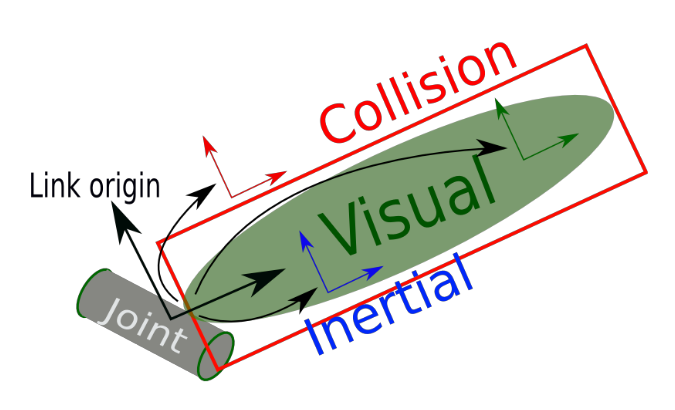
\includegraphics[width = 0.4\linewidth]{image/link标签.png}
\end{figure}

从图中可以看出,检测碰撞的link区域大于外观可视的区域,这就意味着只要有其他物体与collision区域相交,就认为link发生碰撞。

<link>标签的一般结构如下:

\begin{verbatim}
    <link name = "<name of the link>">
        <inertial> ...... </inertial>
        <visual> ...... </visual>
        <collision> ...... </collision>
    </link>
\end{verbatim}

其中:
\begin{itemize}
    \item <visual>:用于描述机器人link部分的外观参数
    \item <inertial>:用于描述link的惯性参数
    \item <collision>:用于描述link的碰撞部分
\end{itemize}

\subsection{<joint>标签}\label{subsec:joint}

<joint>标签用于描述机器人关节的运动学和动力学属性,包括关节运动的位置和速度限制。根据机器人的关节运动形式,可以将其分为六种类型:

\begin{table}[H]
    \centering
    \begin{tabular}{c|c}
    \hline
    \textbf{关节类型} & \textbf{描述}            \\ \hline
    continuous    & 旋转关节,可以围绕单轴无限旋转        \\ \hline
    revolute      & 旋转关节,有旋转的角度限制          \\ \hline
    prismatic     & 滑动关节,沿某一轴线移动的关节,带有位置极限 \\ \hline
    planar        & 平面关节,允许在平面正交方向上平移或者旋转  \\ \hline
    floating      & 浮动关节,允许进行平移、旋转运动       \\ \hline
    fixed         & 固定关节,不允许运动的特殊关节        \\ \hline
    \end{tabular}
\end{table}

机器人关节的主要作用是连接两个刚体link,这两个link分别称为parent link和child link,如下图所示:

\begin{figure}[H]
    \centering
    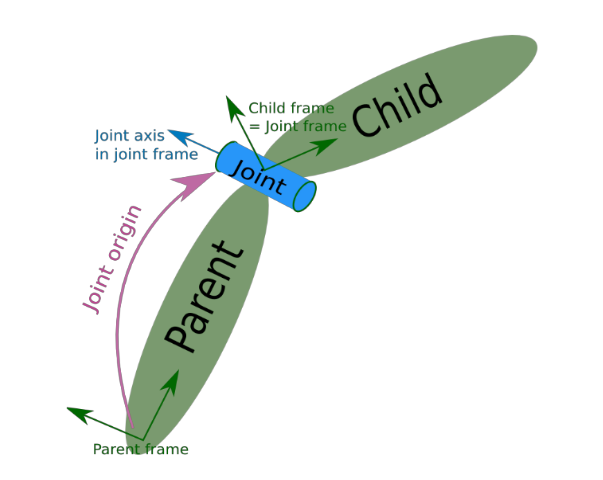
\includegraphics[width = 0.5\linewidth]{image/joint标签.png}
\end{figure}

<link>标签的一般结构如下:

\begin{verbatim}
    <joint name = "<name of the joint>">
        <parent link = "parent_link"/>
        <child link = "child_link"/>
        <calibration .... />
        <dynamics damping .... />
        <limit effort .... />
        ....
    </joint>
\end{verbatim}

其中必须指定joint的parent link和child link,还可以设置关节的其他属性:

\begin{itemize}
    \item <calibration>:关节的参考位置,用来校准关节的绝对位置。
    \item <dynamics>:用于描述关节的物理属性,例如阻尼、静摩擦力,经常在动力学仿真中出现。
    \item <limit>:用于描述运动的一些极限值,包括关节运动的上下限位置、速度限制、力矩限制等。
    \item <mimic>:用于描述该关节与已有关节的关系。
    \item <safety\_controller>:用于描述安全控制器参数。
\end{itemize}

\subsection{<robot>标签}

<robot>是完整机器人模型的最顶层标签,<link>和<joint>标签都必须包含在<robot>标签内。robot标签内可以设置机器人的名称,其基本语法如下:

\begin{verbatim}
    <robot name = "name of the robot">
        <link> ...... </link>
        <link> ...... </link>
        <joint> ...... </joint>
        <joint> ...... </joint>
    </robot>
\end{verbatim}

\subsection{<gazebo>标签}

<gazebo>标签用于描述机器人模型在Gazebo中仿真所需要的参数,包括机器人材料的属性、Gazebo插件。该标签不是机器人模型的必需部分,只有在Gazebo中仿真时才需要加入,其基本语法如下:

\begin{verbatim}
    <gazebo reference = "link_1">
        <material>Gazebo/Black</material>
    </gazebo>
\end{verbatim}

\section{创建URDF模型}

以MRobot机器人为例。

\subsection{创建功能包}

使用如下命令创建一个urdf模型的功能包:

\begin{verbatim}
    $ catkin_create_pkg mrobot_description urdf xacro
\end{verbatim}

创建好的功能包中包含如下四个文件夹:

\begin{itemize}
    \item urdf:用于存放机器人模型的URDF文件或xacro文件
    \item mashes:用于放置URDF中引用的模型渲染文件
    \item launch:用于保存相关启动文件
    \item config:用于保存rviz的配置文件
\end{itemize}

\subsection{URDF模型代码}

\subsubsection{part 1}

\begin{verbatim}
    <?xml version="1.0" ?>
    <robot name="mrobot_chassis">
\end{verbatim}

首先在文件开头,需要生命该文件使用XML描述,然后使用<robot>根标签定义一个机器人模型,并定义机器人的名称。

\subsubsection{part 2}
\begin{verbatim}
    <link name="base_link">
        <visual>
            <origin xyz=" 0 0 0" rpy="0 0 0" />
            <geometry>
                <cylinder length="0.005" radius="0.13"/>
            </geometry>
            <material name="yellow">
                <color rgba="1 0.4 0 1"/>
            </material>
        </visual>
    </link>
\end{verbatim}

这一段代码描述机器人的底盘link,<visual>标签定义底盘的外观属性;

在<geometry>标签下定义几何外观,我们将底盘抽象成一个圆柱,使用<cylinder>标签定义这个圆柱的半径和高;

然后声明这个底盘圆柱在三维坐标位置和旋转姿态,使用<origin>标签设置底盘中心位置,底盘中心位于界面的中心点,所以将坐标设置为“0 0 0”,旋转设置也设置为“0 0 0”即可(圆柱体默认是垂直地面放置的);

另外,使用<material>标签设置底盘的颜色——”黄色“,其中<color>标签定义颜色的RGBA值(这里采用百分数描述,A为透明度参数)。

\subsubsection{part 3}

\begin{verbatim}
    <joint name="base_left_motor_joint" type="fixed">
        <origin xyz="-0.055 0.075 0" rpy="0 0 0" />        
        <parent link="base_link"/>
        <child link="left_motor" />
    </joint>
\end{verbatim}

这一段代码定义一个关节joint,用来连接机器人底盘和左边驱动电机,joint类型为fixed类型,这种类型的joint是固定的(见\autoref{subsec:joint})。

<origin>标签设置了joint的起点,将起点设置在需要安装电机的底盘位置。

\subsubsection{part 4}

\begin{verbatim}
    <link name="left_motor">
        <visual>
            <origin xyz="0 0 0" rpy="1.5707 0 0" />
            <geometry>
                <cylinder radius="0.02" length = "0.08"/>
            </geometry>
            <material name="gray">
                <color rgba="0.75 0.75 0.75 1"/>
            </material>
        </visual>
    </link>
\end{verbatim}

这一段代码描述了左侧电机的模型,外形也是圆柱体,采用<cylinder>标签。

关于<origin>标签的设置:由于我们上面定义了一个joint用来将电机连接到底盘上,电机的位置是相对于joint计算的。在joint的位置设置中,已经将其放置到了安装电机的位置,所以电机模型的位置设置到“0 0 0”坐标就可以了。

另外由于圆柱体默认垂直地面,因此我们需要将电机模型绕x轴旋转90°放置。

\subsubsection{part 5}

\begin{verbatim}
    <joint name="left_wheel_joint" type="continuous">
        <origin xyz="0 0.0485 0" rpy="0 0 0"/>
        <parent link="left_motor"/>
        <child link="left_wheel_link"/>
        <axis xyz="0 1 0"/>
    </joint>
\end{verbatim}

这一段代码定义一个关节joint,用来连接电机和轮子,joint类型为continuous类型,这种类型的joint可以绕一个轴旋转(见\autoref{subsec:joint})。

<origin>标签将轮子的起点设置到电机的一端,<axis>标签定义该joint的旋转轴是y轴。

\subsubsection{添加物理和碰撞属性}

前面的代码仅创建了模型的可视化属性,还需要添加物理属性和碰撞属性,这里以机器人底盘base\_link为例:

\begin{verbatim}
    <link name="base_link">
        <intertial>
            <mass value="2"/>
            <origin xyz="0 0 0.0"/>
            <inertia ixx="0.01" ixy="0.0" ixz="0.0"
                     iyy="0.01" iyz="0.0" 
                     izz="0.5"/>
        </inertial>

        <visual>
            <origin xyz=" 0 0 0" rpy="0 0 0" />
            <geometry>
                <cylinder length="${base_link_length}" radius="${base_link_radius}"/>
            </geometry>
            <material name="yellow">
            </material>
        </visual>

        <collision>
            <origin xyz="0 0 0" rpy="0 0 0"/>
            <geometry>
                <cylinder length="${base_link_length}" radius="${base_link_radius}"/>
            </geometry>
        </collision>
    </link>
\end{verbatim}

其中<intertial>标签设置惯性参数,主要包括质量和惯性矩阵,如果是规则物体,可以通过尺寸、质量等公式计算得到惯性矩阵(这里有待学习补充)。

\section{使用xacro优化URDF模型}

URDF文件不支持代码复用的特性,因此针对URDF模型提出了一种精简化、可复用、模块化的描述形式——xacro。

xacro有两点优点:精简的模型代码、提供可编程接口。模型的后缀名由.urdf变为.xacro,并且需要在模型的<robot>标签中加入xacro的声明,代码如下:

\begin{verbatim}
    <?xml version="1.0"?>
    <robot name="mrobot" xmlns:xacro="http://www.ros.org/wiki/xacro">
\end{verbatim}

\subsection{xacro的三个机制}

\subsubsection{使用常量定义}

定义常量的语法如下:

\begin{verbatim}
    <xacro:property name="M_PI" value="3.14159"/>
\end{verbatim}

使用常量的语法如下:

\begin{verbatim}
    <origin xyz="0 0 0" rpy="${M_PI} 0 0"/>
\end{verbatim}

\subsubsection{调用数学公式}

在”\${}“语句中,不仅可以调用常量,还可以使用一些常用的数学运算,包括加减乘除、负号、括号等(所有运算都会被转换成浮点数进行),语法如下:

\begin{verbatim}
    <origin xyz="0 ${(motor_length+wheel_length)/2} 0" rpy="0 0 0"/>
\end{verbatim}

\subsubsection{使用宏定义}

xacro文件可以使用宏定义来声明重复使用的代码模块,而且可以包含输入参数,以MRobot机器人的八根支撑柱为例,宏定义的语法示例如下:

\begin{verbatim}
    <xacro:macro name="mrobot_standoff_2in" params="parent number x_loc y_loc z_loc">
        <joint name="standoff_2in_${number}_joint" type="fixed">
            <origin xyz="${x_loc} ${y_loc} ${z_loc}" rpy="0 0 0" />
            <parent link="${parent}"/>
            <child link="standoff_2in_${number}_link" />
        </joint>

        <link name="standoff_2in_${number}_link">
            <inertial>
                <mass value="0.001" />
                <origin xyz="0 0 0" />
                <inertia ixx="0.0001" ixy="0.0" ixz="0.0"
                         iyy="0.0001" iyz="0.0"
                         izz="0.0001" />
            </inertial>

            <visual>
                <origin xyz=" 0 0 0 " rpy="0 0 0" />
                <geometry>
                    <box size="0.01 0.01 0.07" />
                </geometry>
                <material name="black">
                    <color rgba="0.16 0.17 0.15 0.9"/>
                </material>
            </visual>

            <collision>
                <origin xyz="0.0 0.0 0.0" rpy="0 0 0" />
                <geometry>
                    <box size="0.01 0.01 0.07" />
                </geometry>
            </collision>
        </link>
    </xacro:macro>
\end{verbatim}

以上的宏定义包含五个输入参数:joint的parent link,支撑住的序号,支撑柱在xyz三个方向上的偏移。这个宏定义在定义一个支撑柱的时候,分别对其joint和link两个标签进行了定义。

当需要使用该宏模块的时候,按照如下语法进行调用:

\begin{verbatim}
    <mrobot_standoff_2in parent="base_link" number="1" x_loc="-${standoff_x/2 + 0.03}" 
y_loc="-${standoff_y - 0.03}" z_loc="${plate_height/2}"/>
\end{verbatim}


\subsection{引用xacro文件}

引用示例如下:

\begin{verbatim}
    <?xml version="1.0"?>
    <robot name="mrobot" xmlns:xacro="http://www.ros.org/wiki/xacro">
        <xacro:include filename="$(find mrobot_description)/urdf/mrobot_body.urdf
    .xacro" />
        <!-- MRobot机器人平台 -->
        <mrobot_body/>
    </robot>
\end{verbatim}

可以看到,在robot标签之间,首先使用了xacro:inlude标签,包含了另一个xacro模型文件,然后我们就可以在下面使用被包含文件中的模块了。接下来调用被包含文件中的机器人模型宏定义(机器人模型文件全部是在被包含文件中用一个宏来描述的)。

这样将整个机器人模型作为一个宏有什么好处呢?把机器人整体看做一个模块,方便与其他模型进行集成,比如在后续安装传感器等其他模块时。

\subsection{显示xacro优化后的模型}

\subsubsection{将xacro文件转化成URDF文件}

使用如下命令可以将xacro文件转换成URDF文件:

\begin{verbatim}
    $ rosrun xacro xacro.py mrobot.urdf.xacro > mrobot.urdf
\end{verbatim}

\subsubsection{直接调用xacro文件解析器}

也可以省略手动转换的过程,直接在启动文件中调用xacro解析器,自动将xacro转换成URDF文件,在launch文件中使用如下语句进行配置:

\begin{verbatim}
    <arg name="model" default="$(find xacro)/xacro --inorder '$(find mrobot_description)/urdf/mrobot.urdf.xacro'" />
	<arg name="gui" default="true" />
\end{verbatim}

进而可以直接使用这个修改后的启动文件,看到xacro格式的机器人模型。

\section{添加传感器模型}

首先我们需要自己创建一个传感器模型(xacro文件),或者去网上下载一个传感器的模型,这里以一个摄像头为例,其模型文件为camera.xacro。

进而我们可以创建一个顶层xacro文件,将机器人主体与摄像头连接起来:

\begin{verbatim}
    <?xml version="1.0"?>
    <robot name="mrobot" xmlns:xacro="http://www.ros.org/wiki/xacro">

        <xacro:include filename="$(find mrobot_description)/urdf/mrobot_body.urdf
    .xacro" />
        <xacro:include filename="$(find mrobot_description)/urdf/camera.xacro" />

        <xacro:property name="camera_offset_x" value="0.1" />
        <xacro:property name="camera_offset_y" value="0" />
        <xacro:property name="camera_offset_z" value="0.02" />

        <!-- MRobot机器人平台-->
        <mrobot_body/>

        <!-- Camera -->
        <joint name="camera_joint" type="fixed">
            <origin xyz="${camera_offset_x} ${camera_offset_y} ${camera_offset_z}" rpy="0 0 0" />
            <parent link="plate_2_link"/>
            <child link="camera_link"/>
        </joint>

        <xacro:usb_camera prefix="camera"/>

    </robot>
\end{verbatim}

在这个顶层文件中,包含了描述摄像头的模型文件以及描述机器人的模型文件,然后使用了一个fixed类型的joint把摄像头固定到机器人的指定位置。

\section{基于ArbotiX和rviz的仿真器}

ArbotiX提供一个差速控制器,通过接收速度控制指令更新机器人的joint状态,从而实现机器人在rviz中的运动。

\subsection{在ROS-melodic中安装ArbotiX}

Arbotix本质上就是一个功能包,我们需要像其他我们自己的功能包一样,将其放置在工作空间下的src目录下,直接从git上下载其源码:

\begin{verbatim}
    $ git clone -b indigo-devel https://github.com/vanadiumlabs/arbotix_ros.git
\end{verbatim}

然后重新编译工程即可(注意如果没有将设置环境变量的指令放到.bashrc中,在这里要记得使用source命令设置环境变量)。

\subsection{配置ArbotiX控制器}

我们只需要适当修改原本的launch文件,然后再创建一个控制器相关的配置文件就可以了。

\subsubsection{修改launch文件}

只是在显示机器人模型的launch文件的基础上加上如下内容:

\begin{verbatim}
    <node name="arbotix" pkg="arbotix_python" type="arbotix_driver" output="screen">
        <rosparam file="$(find mrobot_description)/config/fake_mrobot_arbotix.yaml" 
    command="load" />
        <param name="sim" value="true"/>
    </node>
\end{verbatim}

从以上代码可以看出,实际上就是添加了一个控制器节点,这里在仿真环境中使用,需要配置“sim”参数为true。另外,从这里可以看到,启动时还需要加载一个叫“fake\_mrobot\_arbotix.yaml”的配置文件。

\subsubsection{创建配置文件}

配置文件的目录为:功能包目录/config/下,文件内容如下:

\begin{verbatim}
    controllers: {
        base_controller: {
            type: diff_controller, 
            base_frame_id: base_footprint, 
            base_width: 0.26, 
            ticks_meter: 4100, 
            Kp: 12, 
            Kd: 12, 
            Ki: 0, 
            Ko: 50, 
            accel_limit: 1.0 
        }
    }
\end{verbatim}

控制器的名称为“base\_controller”,类型为“diff\_controller”(差速控制器),另外还给出了参考坐标系、底盘尺寸、PID参数等。

\subsection{运行仿真}

需要注意的是,我们要设置参考坐标系(fixed frame)为“odom”,才可以看到小车的移动。

\section{ros\_control}

ros\_control是一套机器人控制中间件,包含一系列控制器接口、传动装置接口、硬件接口、控制器工具箱等。

\subsection{ros\_control的框架}

\begin{figure}[H]
    \centering
    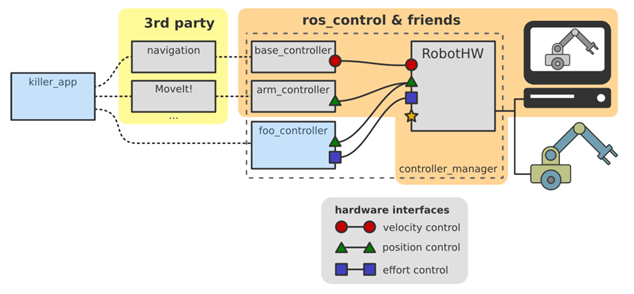
\includegraphics[width=0.8\linewidth]{image/ros_control.png}
\end{figure}

上图是ros\_control的总体框架,可以看到正对不同类型的控制器(底盘、机械臂等),ros\_control可以提供多种类型的控制器,但是这些控制器的接口各不相同,为了提高代码的复用率,ros\_control还提供一个硬件的抽象层。硬件抽象层负责机器人硬件资源的管理,而controller从抽象层请求资源即可,并不直接接触硬件。

\subsection{控制器}

ROS的ros\_controllers功能包提供了一些常用的控制器:

\begin{itemize}
    \item effort\_controllers
        \begin{itemize}
            \item joint\_effort\_controller
            \item joint\_position\_controller
            \item joint\_velocity\_controller
        \end{itemize}
    \item joint\_state\_controller
        \begin{itemize}
            \item joint\_state\_controller
        \end{itemize}
    \item position\_controllers
        \begin{itemize}
            \item joint\_position\_controller
        \end{itemize}
    \item velocity\_controllers
        \begin{itemize}
            \item joint\_velocity\_controller
        \end{itemize}
\end{itemize}

另外,也可以根据自己的需求创建需要的控制器,并通过控制器管理器进行管理(具体方法有需要再补充)。

\subsection{硬件接口}

\begin{figure}[H]
    \centering
    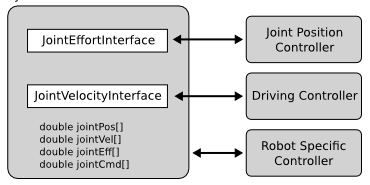
\includegraphics[width=0.4\linewidth]{image/硬件接口.png}
\end{figure}

硬件接口是控制器与RobotHW(硬件抽象层)沟通的接口,基本与控制器种类相对应。另外也可以根据自己的需求创建需要的接口(具体方法有需要再补充)。

\subsection{传动系统}

\subsection{关节约束}

\subsection{控制器管理器}


\section{Gazebo仿真}






































































































































































































































































































































































































































































































































































































\end{document}

